\documentclass{article}
\usepackage{tikz}
\usepackage{amsmath}
\usepackage[margin=0pt,paperwidth=32cm,paperheight=21cm]{geometry}
\usetikzlibrary{calc,patterns,arrows.meta}
\pagestyle{empty}
\begin{document}
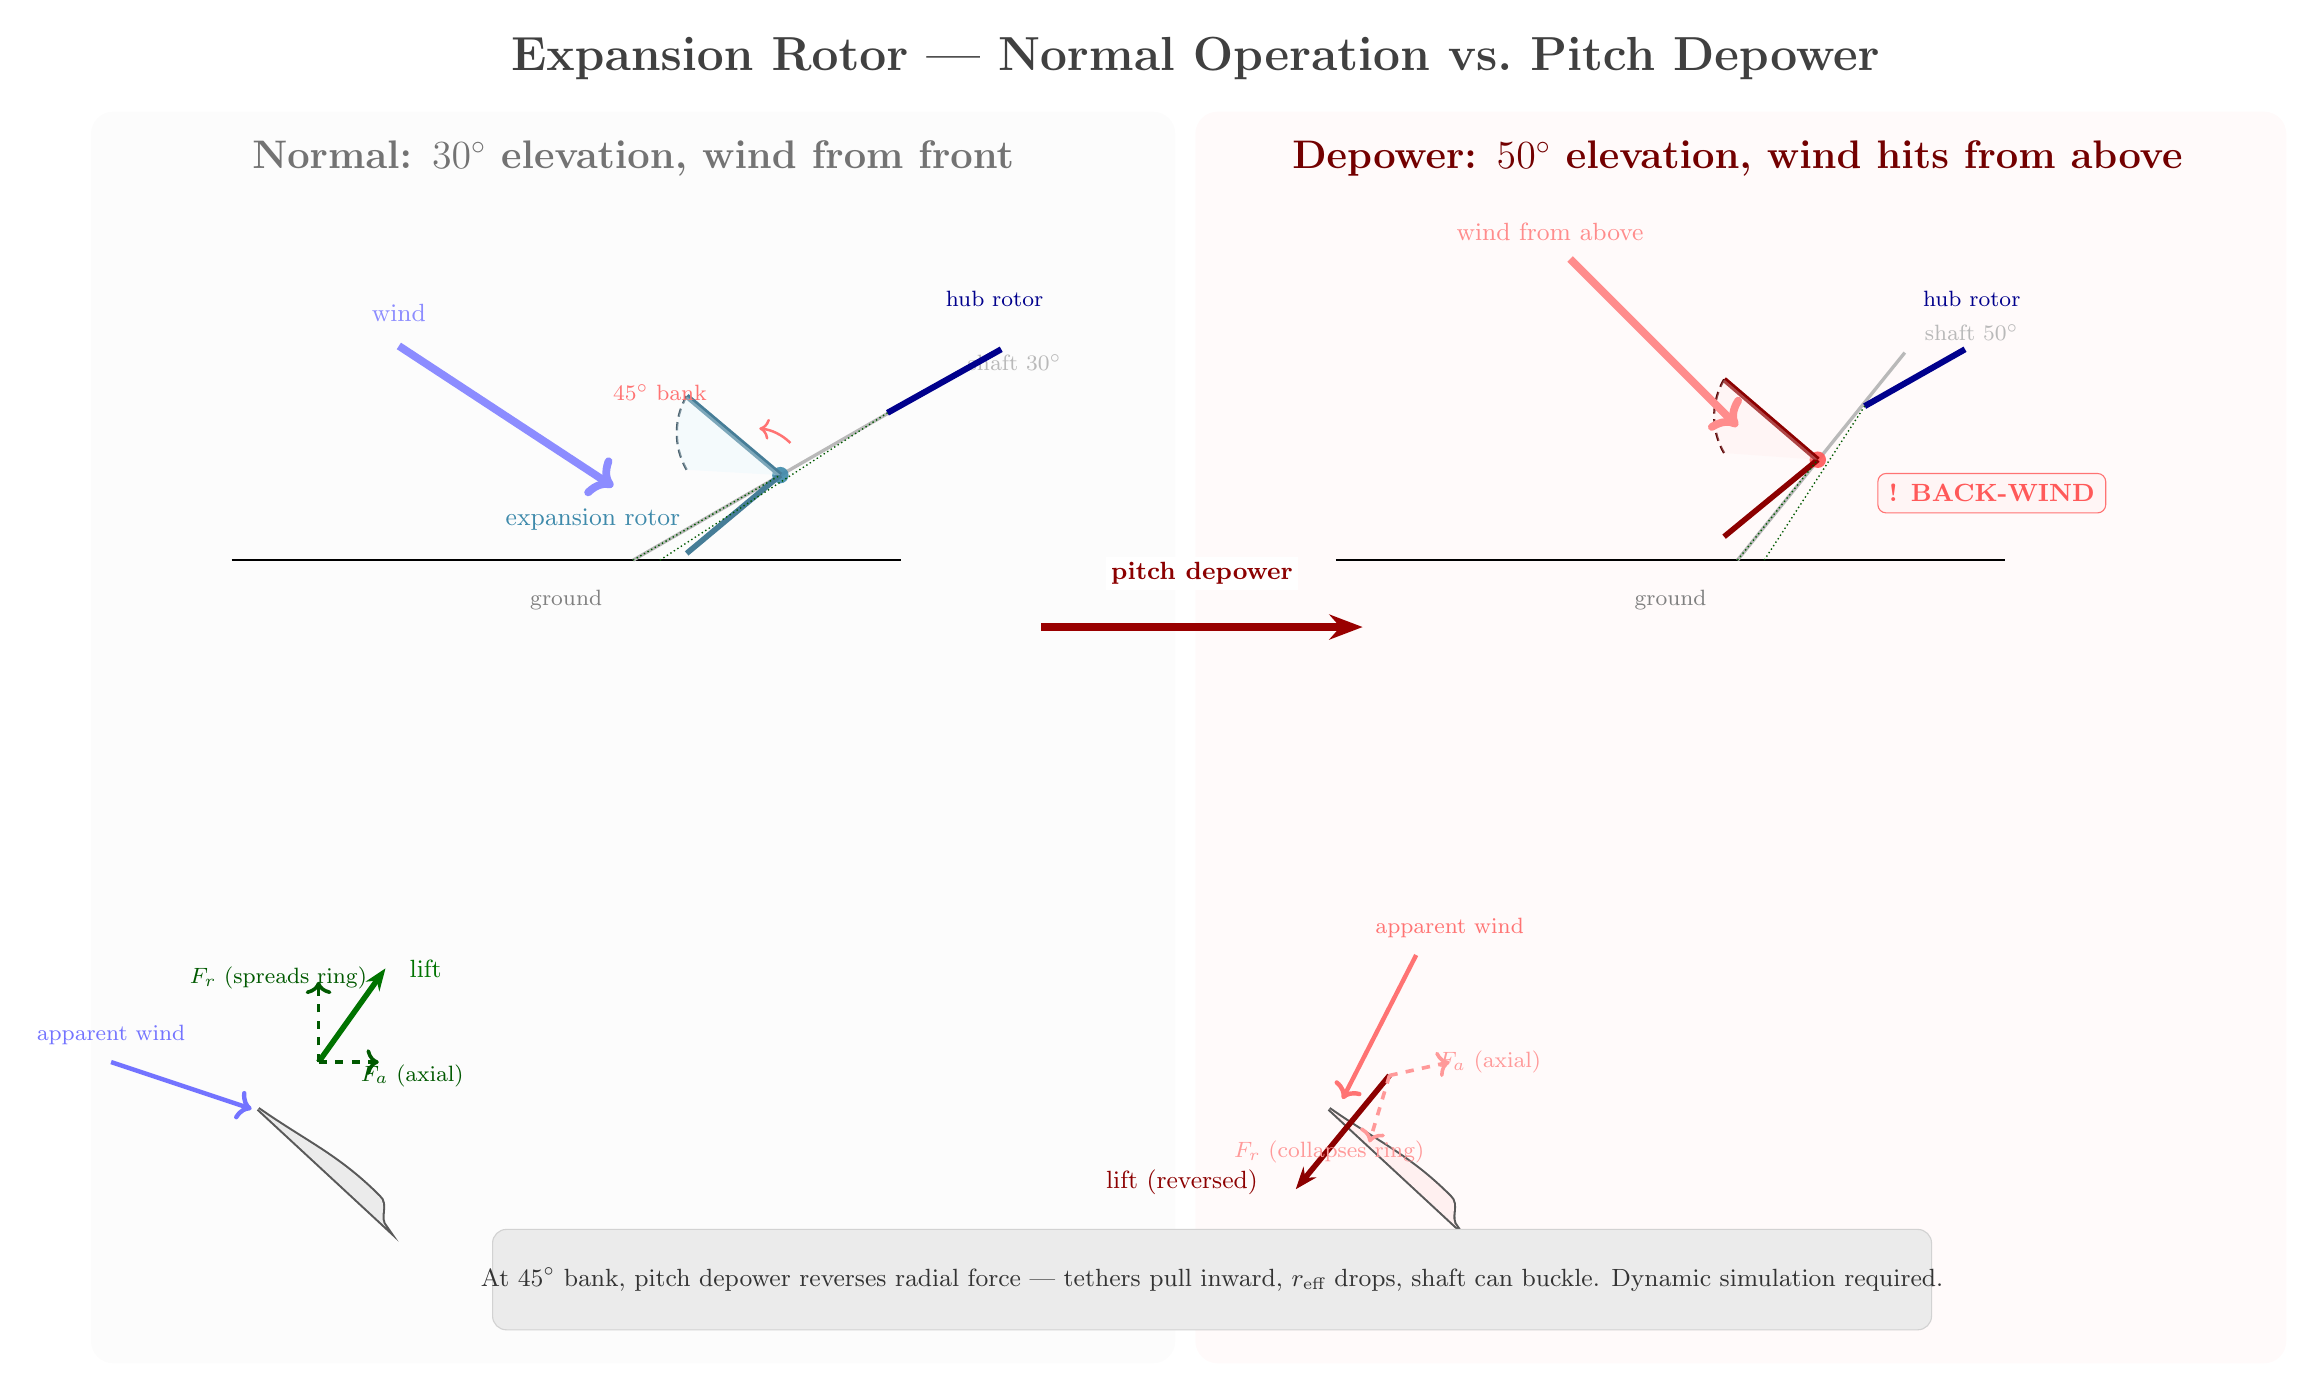
\begin{tikzpicture}[scale=0.85]

% ============================================================
% TITLE
% ============================================================
\node[font=\bfseries\LARGE, black!75] at (15.5,19.0) {Expansion Rotor — Normal Operation vs.\ Pitch Depower};

% ============================================================
% PANEL BACKGROUNDS (drawn first so transition arrow sits on top)
% ============================================================
\fill[black!1, rounded corners=8pt] (-1,-0.5) rectangle (15.2,18.2);
\node[font=\bfseries\Large, black!55] at (7.1,17.5) {Normal: $30^\circ$ elevation, wind from front};

\fill[red!2, rounded corners=8pt] (15.5,-0.5) rectangle (31.8,18.2);
\node[font=\bfseries\Large, red!45!black] at (23.6,17.5) {Depower: $50^\circ$ elevation, wind hits from above};

% TRANSITION ARROW (on top of both backgrounds)
\draw[->, red!60!black, line width=3pt, arrows={-Stealth[length=12pt,width=9pt]}] (13.2,10.5) -- (18.0,10.5);
\node[font=\bfseries\small, red!55!black, fill=white, inner sep=2pt] at (15.6,11.3) {pitch depower};

% ============================================================
% LEFT PANEL CONTENT
% ============================================================
\begin{scope}[shift={(7.1,11.5)}]
  % Ground
  \draw[thick] (-6.0,0) -- (4.0,0);
  \node[font=\footnotesize, black!50] at (-1.0,-0.6) {ground};

  % Shaft at 30°
  \draw[gray!55, line width=1.2pt] (0,0) -- (4.6,2.65);
  \node[font=\footnotesize, gray!55] at (5.7,2.95) {shaft $30^\circ$};

  % Hub rotor
  \draw[blue!55!black, line width=2.2pt] (3.8,2.2) -- (5.5,3.15);
  \node[font=\footnotesize, blue!55!black] at (5.4,3.9) {hub rotor};

  % Expansion rotor at ring — hub point on shaft
  \fill[cyan!65!black, opacity=0.9] (2.2,1.27) circle (3.5pt);

  % Blade extending at 45° bank — upper side
  \draw[cyan!55!black, line width=2.0pt] (2.2,1.27) -- (0.8,2.45);
  % Blade — lower side
  \draw[cyan!55!black, line width=2.0pt] (2.2,1.27) -- (0.8,0.1);

  % Cone swept surface (dashed arc + translucent fill)
  \draw[cyan!35!black, line width=0.8pt, densely dashed] (0.8,2.45) arc (150:210:1.1);
  \fill[cyan!10, opacity=0.35] (2.2,1.27) -- (0.8,2.45) arc (150:210:1.1) -- cycle;

  % Bank angle arc
  \draw[->, red!55, line width=0.9pt] (2.0,1.55) ++(0.35,0.2) arc (45:85:0.75);
  \node[font=\footnotesize, red!55] at (0.4,2.5) {$45^\circ$ bank};

  % Wind arrow — from left/front
  \draw[->, blue!45, line width=2.8pt] (-3.5,3.2) -- (-0.3,1.1);
  \node[font=\small, blue!45] at (-3.5,3.7) {wind};

  % Label
  \node[font=\small, cyan!65!black] at (-0.6,0.6) {expansion rotor};

  % Tether lines
  \draw[green!35!black, line width=0.5pt, densely dotted] (0,0) -- (2.2,1.27);
  \draw[green!35!black, line width=0.5pt, densely dotted] (0.4,0) -- (3.8,2.2);
\end{scope}

% Blade cross-section — normal (shifted right to avoid edge)
\begin{scope}[shift={(1.5,3.3)}]
  % Airfoil at 45° bank
  \draw[black!65, line width=1.5pt, rotate around={-45:(0,0)}]
    (0,0) to[out=10, in=180] (2.2,0.35) to[out=5, in=180] (2.6,0.1) -- cycle;
  \fill[black!8, rotate around={-45:(0,0)}] (0,0) to[out=10, in=180] (2.2,0.35) to[out=5, in=180] (2.6,0.1) -- cycle;

  % Apparent wind
  \draw[->, blue!55, line width=1.6pt] (-2.2,0.7) -- (-0.1,0.0);
  \node[font=\footnotesize, blue!55] at (-2.2,1.1) {apparent wind};

  % Lift vector
  \draw[->, green!45!black, line width=2.0pt, arrows={-Stealth[length=8pt,width=6pt]}] (0.9,0.7) -- (1.9,2.1);
  \node[font=\small, green!45!black] at (2.5,2.1) {lift};

  % Force decomposition
  \draw[->, green!35!black, line width=1.3pt, dashed] (0.9,0.7) -- (0.9,1.9);
  \node[font=\footnotesize, green!35!black] at (0.3,1.95) {$F_r$ (spreads ring)};

  \draw[->, green!35!black, line width=1.3pt, dashed] (0.9,0.7) -- (1.8,0.7);
  \node[font=\footnotesize, green!35!black] at (2.3,0.5) {$F_a$ (axial)};
\end{scope}

% ============================================================
% RIGHT PANEL CONTENT
% ============================================================
\begin{scope}[shift={(23.6,11.5)}]
  % Ground
  \draw[thick] (-6.0,0) -- (4.0,0);
  \node[font=\footnotesize, black!50] at (-1.0,-0.6) {ground};

  % Shaft at 50°
  \draw[gray!55, line width=1.2pt] (0,0) -- (2.5,3.1);
  \node[font=\footnotesize, gray!55] at (3.5,3.4) {shaft $50^\circ$};

  % Hub rotor
  \draw[blue!55!black, line width=2.2pt] (1.9,2.3) -- (3.4,3.15);
  \node[font=\footnotesize, blue!55!black] at (3.5,3.9) {hub rotor};

  % Expansion rotor hub point
  \fill[red!65, opacity=0.9] (1.2,1.5) circle (3.5pt);

  % Blade — upper
  \draw[red!55!black, line width=2.0pt] (1.2,1.5) -- (-0.2,2.7);
  % Blade — lower
  \draw[red!55!black, line width=2.0pt] (1.2,1.5) -- (-0.2,0.35);

  % Cone swept
  \draw[red!35!black, line width=0.8pt, densely dashed] (-0.2,2.7) arc (150:210:1.1);
  \fill[red!8, opacity=0.3] (1.2,1.5) -- (-0.2,2.7) arc (150:210:1.1) -- cycle;

  % Wind from above
  \draw[->, red!45, line width=2.8pt] (-2.5,4.5) -- (0.0,2.0);
  \node[font=\small, red!45] at (-2.8,4.9) {wind from above};

  % BACK-WIND warning
  \node[font=\bfseries\small, red!65, fill=red!4, draw=red!55, rounded corners=3pt, inner sep=4pt] at (3.8,1.0) {! BACK-WIND};

  % Tether lines
  \draw[green!35!black, line width=0.5pt, densely dotted] (0,0) -- (1.2,1.5);
  \draw[green!35!black, line width=0.5pt, densely dotted] (0.4,0) -- (1.9,2.3);
\end{scope}

% Blade cross-section — back-winded (shifted right to avoid left edge)
\begin{scope}[shift={(17.5,3.3)}]
  % Airfoil (same orientation)
  \draw[black!65, line width=1.5pt, rotate around={-45:(0,0)}]
    (0,0) to[out=10, in=180] (2.2,0.35) to[out=5, in=180] (2.6,0.1) -- cycle;
  \fill[red!6, rotate around={-45:(0,0)}] (0,0) to[out=10, in=180] (2.2,0.35) to[out=5, in=180] (2.6,0.1) -- cycle;

  % Apparent wind from above
  \draw[->, red!55, line width=1.6pt] (1.3,2.3) -- (0.2,0.15);
  \node[font=\footnotesize, red!55] at (1.8,2.7) {apparent wind};

  % Lift REVERSED — extend further down-left to make space for labels
  \draw[->, red!55!black, line width=2.0pt, arrows={-Stealth[length=8pt,width=6pt]}] (0.9,0.5) -- (-0.5,-1.2);
  \node[font=\small, red!55!black] at (-2.2,-1.1) {lift (reversed)};

  % Force decomposition — spread apart from lift arrow
  \draw[->, red!40, line width=1.3pt, dashed] (0.9,0.5) -- (0.6,-0.5);
  \node[font=\footnotesize, red!40] at (0.0,-0.65) {$F_r$ (collapses ring)};

  \draw[->, red!40, line width=1.3pt, dashed] (0.9,0.5) -- (1.8,0.7);
  \node[font=\footnotesize, red!40] at (2.4,0.7) {$F_a$ (axial)};
\end{scope}

% ============================================================
% BOTTOM: Key takeaway
% ============================================================
\fill[black!8, draw=gray!35, rounded corners=5pt] (5.0,0.0) rectangle (26.5,1.5);
\node[font=\small, black!80, align=center] at (15.75,0.75) {At $45^\circ$ bank, pitch depower reverses radial force — tethers pull inward, $r_{\text{eff}}$ drops, shaft can buckle. Dynamic simulation required.};

\end{tikzpicture}
\end{document}
